\documentclass[12pt, a4paper]{article}

% --- Encoding & Fonts ---
\usepackage[T1]{fontenc}
\usepackage[utf8]{inputenc}
\usepackage{lmodern}

% --- Page Layout ---
\usepackage[margin=1in]{geometry}

% --- Math ---
\usepackage{amsmath, amssymb}

% --- Graphics & Figures ---
\usepackage{graphicx}
\usepackage{float}
\usepackage[export]{adjustbox}

% --- Diagrams ---
\usepackage{tikz}
\usepackage{pgfplots}
\pgfplotsset{compat=1.18}
\usetikzlibrary{arrows.meta, positioning, shapes.geometric, calc}

% --- Tables ---
\usepackage{booktabs}
\usepackage{longtable}
\usepackage{tabularx}
\usepackage{array}

% --- Hyperlinks ---
\usepackage[
    colorlinks=true,
    linkcolor=blue!70!black,
    citecolor=green!50!black,
    urlcolor=blue!60!black,
    bookmarks=true
]{hyperref}

% --- Bibliography ---
\usepackage[
    backend=biber,
    style=numeric-comp,
    sorting=none,
    maxbibnames=3,
    minbibnames=1,
    url=true,
    doi=false,
    eprint=false
]{biblatex}
\addbibresource{references.bib}

% --- Misc ---
\usepackage{microtype}
\usepackage{xcolor}
\usepackage{enumitem}
\usepackage{eurosym}
\setlength{\parskip}{0.5em}
\setlength{\parindent}{0pt}
\raggedbottom

% --- User customizations ---
\usepackage{amsthm}
\geometry{top=2.5cm, bottom=2.5cm, left=3cm, right=3cm}

% --- Metadata ---
\title{Navegación Autónoma Híbrida en BEV con Optimización de Rutas para Seguimiento de Cultivos}
\author{Pedro Canales}
\date{19 August 2026}

\begin{document}
\maketitle
\tableofcontents
\newpage

\%\% ============================================================
\%\% TITLE PAGE
\%\% ============================================================
\begin{titlepage}
\centering
\vspace*{2.5cm}

{\LARGE\bfseries Navegación Autónoma Híbrida en BEV con\\[6pt]
Optimización de Rutas para Seguimiento de Cultivos\par}

\vspace{0.9cm}
{\large\itshape Hybrid Autonomous Navigation Based on BEV Representations\\[3pt]
and Constrained Optimisation for Crop Tracking and Identification\par}

\vspace{2.8cm}
{\large Pedro Canales\par}

\vspace{1.5cm}
{\normalsize Master's Thesis\par}
\vspace{0.4cm}
{\normalsize 19 August 2026\par}

\vfill
\end{titlepage}

\%\% ============================================================
\%\% ABSTRACT
\%\% ============================================================
\begin{abstract}
Autonomous agricultural robotics faces a tripartite challenge: perceiving complex,
unstructured field environments in a representation suitable for motion planning; generating
safe, complete, and energy-efficient coverage trajectories under stringent vehicle and
implement constraints; and identifying crop-health anomalies in real time so that route
priorities can be adjusted dynamically. Existing literature addresses each of these pillars
in isolation---Bird's-Eye View (BEV) perception advances driven by urban autonomous
driving, coverage path planning rooted in classical computational geometry, and agricultural
computer vision built on crop-disease image benchmarks---yet no integrated system bridges
all three within the resource envelope of an agricultural prototype platform.

This thesis, \emph{Navegación Autónoma Híbrida en BEV con Optimización de Rutas para
Seguimiento de Cultivos}, proposes and evaluates a modular autonomous agricultural vehicle
system that unifies multimodal BEV perception, hybrid classical-plus-learned path planning,
and crop-health computer vision within a cohesive software architecture. The perception
module implements a compact BEV Transformer comprising two parallel convolutional encoder
branches for RGB camera and rasterised LiDAR inputs, fused through bidirectional eight-head
cross-attention into a $200\!\times\!200$ BEV grid with 128 feature channels. Perception
heads produce binary occupancy, six-class semantic segmentation, confidence, and detection
outputs. The planning module combines a classical Boustrophedon global coverage planner with
a lattice-based local planner that scores twenty-step candidate trajectories using a learned
scorer weighted at $\alpha\!=\!0.65$ against a classical cost, and an inflated-cell safety
gate that invokes a stationary fallback when no collision-free trajectory exists.
Trajectory execution is handled by a solver-free, sampled MPC-like kinematic bicycle
controller with a $1.2$\,m wheelbase, twelve-step horizon, and explicit steering and
acceleration limits. Crop identification employs a DeepLabV3+ model with an EfficientNet-B4
encoder, with a torchvision fallback when the preferred dependency is unavailable.

The prototype was trained on 2,000 synthetic samples and evaluated in simulation.
Aggregate results show BEV mIoU exceeding 0.70, hybrid planner collision-free rate above
95\%, MPC trajectory-tracking RMSE below 0.5\,m, crop-identification validation mIoU above
0.70, and full-pipeline throughput above 5\,Hz. These results are simulation- and
prototype-level; field validation on real agricultural terrain has not been established by
the available evidence. The thesis identifies five critical research gaps---absence of
agricultural BEV benchmarks, lightweight embedded BEV perception, ground-vehicle crop-health
BEV integration, hybrid coverage planning with simultaneous health monitoring, and domain
adaptation protocols---and proposes four targeted research questions. Contributions include
a validated modular architecture, a characterised lightweight BEV pipeline, a crop-health
BEV integration method, and a reproducible experimental dataset and evaluation protocol
calibrated to the constraints of an academic prototype.
\end{abstract}

\vspace{1em}
\noindent\textbf{Keywords:} BEV, Transformers, Hybrid Planning, MPC, Agricultural Robotics,
Computer Vision

\listoffigures
\listoftables

\%\% ============================================================
\%\% CHAPTER 1: INTRODUCTION
\%\% ============================================================
\chapter{Introduction}
\label{ch:introduction}

\section{Context and Motivation}

Global agriculture faces mounting pressure to produce more food with fewer inputs, less
environmental impact, and a shrinking rural labour force~\cite{ref138}. Autonomous ground
vehicles offer a pathway to precision crop management: they can operate continuously,
maintain centimetre-level path accuracy, and carry sensor payloads capable of detecting
early-stage crop disease, invasive weeds, and soil anomalies~\cite{ref2, ref32}. Yet
achieving genuine field autonomy---safe navigation through unstructured environments,
guaranteed coverage of irregular field geometries, and real-time identification of
agronomically relevant crop features---requires the integration of three research streams
that have historically developed in isolation.

The first stream is Bird's-Eye View (BEV) perception, where transformer-based architectures
such as BEVFormer~\cite{ref48, ref49} and BEVFusion~\cite{ref13, ref18} have dramatically
improved the ability to fuse heterogeneous sensor modalities into a unified metric top-down
map of the environment. The second is hybrid path planning, where classical coverage path
planners provide formal coverage guarantees while learned local trajectory scorers and
Model Predictive Control (MPC) trackers handle obstacle avoidance and kinematic constraint
satisfaction~\cite{ref103, ref105, ref118}. The third is agricultural computer vision, where
deep learning architectures trained on datasets such as PlantVillage~\cite{ref157, ref159}
and DeepWeeds~\cite{ref167, ref168} can identify crop diseases and weed infestations from
ground-level imagery~\cite{ref149, ref150, ref154}.

A fundamental motivation for integrating these streams is that crop-health observations,
registered in a persistent BEV map, can directly inform the route planner: zones with
detected anomalies can be prioritised for slower, more detailed inspection passes, while
healthy zones can be traversed at operational speed. This closed loop between perception
and planning---where perception informs planning and planning determines what is
observed---represents the core architectural innovation of this thesis.

\section{Problem Statement}

No publicly available system integrates multimodal BEV perception, hybrid coverage
planning, and agricultural crop-health identification in a single architecture validated on
a prototype ground vehicle. The principal obstacles are: (1) the domain gap between urban
BEV benchmarks and agricultural scenes~\cite{ref2, ref32, ref35}; (2) the computational
constraints of agricultural embedded platforms~\cite{ref1}; (3) the absence of
ground-vehicle BEV occupancy datasets for agricultural environments~\cite{ref40}; and
(4) the lack of protocols for integrating crop-health detections into BEV-registered route
cost functions.

\section{Research Objectives and Questions}

This thesis addresses four research questions derived from the identified gaps:

\begin{description}
  \item[RQ1] Can a compact BEV occupancy representation, derived from dual-modality camera
  and LiDAR data on a prototype platform, provide sufficient scene understanding for safe
  agricultural coverage planning?
  \item[RQ2] Does a hybrid classical-plus-learned planning architecture---Boustrophedon CPP
  with lattice-based local planning and sampled MPC tracking---achieve a collision-free rate
  above 95\% and trajectory-tracking RMSE below 0.5\,m in simulation?
  \item[RQ3] Can a DeepLabV3+ crop-health identifier, trained on publicly available
  datasets and domain-adapted to field conditions, achieve validation mIoU above 0.70
  within the resource envelope of the prototype?
  \item[RQ4] Can the integrated pipeline sustain full-stack throughput above 5\,Hz in
  simulation, enabling real-time closed-loop operation?
\end{description}

\section{Scope and Assumptions}

The prototype operates on a single vehicle on known field geometry with static obstacles.
Dynamic obstacles, multi-vehicle coordination, and automatic implement docking are
explicitly out of scope~\cite{ref3}. Validation is simulation- and prototype-level; field
validation on real agricultural terrain has not been established by the available
evidence~\cite{ref234}. All results are aggregate; per-class breakdowns, per-scenario
analyses, ablation studies, and statistical significance tests were not recorded in the
supplied evidence and are recommended for future reproducibility campaigns.

\section{Thesis Organisation}

Chapter~\ref{ch:litreview} synthesises relevant literature across BEV perception, hybrid
planning, and agricultural computer vision, and identifies critical research gaps.
Chapter~\ref{ch:methodology} presents the proposed system architecture and design
decisions. Chapter~\ref{ch:implementation} describes the prototype implementation in
detail. Chapter~\ref{ch:results} reports experimental results. Chapter~\ref{ch:discussion}
interprets those results and identifies limitations. Chapter~\ref{ch:conclusions} states
conclusions and future work. Appendices provide mathematical derivations, implementation
details, and an extended evaluation protocol.

\%\% ============================================================
\%\% CHAPTER 2: LITERATURE REVIEW
\%\% ============================================================
\chapter{Literature Review}
\label{ch:litreview}

\section{Overview and Scope}

This review covers literature directly relevant to an autonomous agricultural vehicle
capable of (a) perceiving its environment as a unified BEV representation from multiple
sensors, (b) planning and executing coverage routes that respect vehicle geometry and
operational constraints, and (c) identifying crop-health patterns in real time. The thesis
scope is deliberately bounded to a Minimum Viable Prototype (MVP) architecture validated
first in simulation, then on a physical platform~\cite{ref1}. Production-grade real-time
BEV inference, multi-vehicle fleet management, and autonomous implement docking are treated
as directions for future development~\cite{ref3}. Sources are synthesised thematically,
with explicit note of areas of agreement or disagreement. The review explicitly
distinguishes established results from single-source claims and from thesis-level
projections.

\section{BEV Transformer Perception}

\subsection{The BEV Representation Paradigm}

The Bird's-Eye View representation has become the dominant spatial encoding in autonomous
driving perception because it provides a metric top-down map in which vehicle geometry,
obstacle extents, and traversability are naturally expressed. Rather than reasoning in
perspective-view image space, a BEV encoder converts heterogeneous sensor observations
into a shared planar or volumetric feature grid aligned with world coordinates. This
alignment is particularly valuable for path planning: the planning module can directly
query the BEV grid for free space and obstacle locations without further geometric
transformation~\cite{ref2, ref3}. The fundamental challenge is \emph{view transformation}:
projecting 2D image features into a 3D or BEV coordinate frame requires either explicit
depth estimation, geometric lifting, or implicit attention-based querying. Different
architectures address this challenge through distinct mechanisms, each with well-documented
trade-offs in accuracy, computational cost, and robustness to sensor
miscalibration~\cite{ref13, ref48, ref49}.

\subsection{Foundational Camera-Only Architectures}

\subsubsection{BEVFormer}

BEVFormer~\cite{ref48, ref49} introduced a spatiotemporal transformer architecture in which
a fixed grid of learnable BEV queries interacts with multi-view image features through two
purpose-built attention mechanisms. The \emph{spatial cross-attention} module associates
each BEV query with regions of interest across all camera views, implementing a form of
implicit epipolar geometry without requiring explicit depth prediction. The \emph{temporal
self-attention} module recurrently fuses BEV feature maps from previous time steps,
operating analogously to an RNN hidden state to propagate motion and occlusion cues across
frames~\cite{ref49}. This architecture was reported to achieve 56.9\% NDS on the nuScenes
test set, substantially outperforming prior methods such as DETR3D, and is particularly
noted for improved velocity estimation and object recall under low-visibility
conditions~\cite{ref48}. Subsequent variants have extended BEVFormer with gated
transformer layers for instance prediction (BEVPredFormer~\cite{ref51}) and with
learning-first view attention to relax sensor deployment constraints
(ViewFormer~\cite{ref57}).

\subsubsection{BEVDet and BEVDet4D}

BEVDet and its temporal extension BEVDet4D employ the Lift-Splat-Shoot (LSS) module for
2D-to-3D feature transformation, offering higher computational efficiency than the
attention-heavy BEVFormer design~\cite{ref7, ref8}. BEVDet4D augments the single-frame
approach by preserving and concatenating BEV feature maps from preceding frames, capturing
temporal clues for velocity estimation and handling of briefly occluded
objects~\cite{ref7, ref8, ref16, ref18}. The LSS mechanism explicitly discretises the camera
frustum and distributes pixel-level features into a voxel grid using predicted categorical
depth distributions, which makes depth prediction quality a critical
bottleneck~\cite{ref7, ref8}.

\subsubsection{PETR and StreamPETR}

PETR (Position Embedding Transformation) replaces complex online 2D-to-3D feature
sampling with a coordinate-based approach~\cite{ref66, ref67}. The camera frustum space is
discretised into a 3D mesh-grid, transformed into world coordinates using calibrated
camera parameters, and these coordinates are encoded into the 2D image features extracted
by a backbone network. The resulting 3D position-aware features allow object queries to
perform end-to-end detection directly in the 3D domain through a transformer decoder,
avoiding inaccurate reference-point sampling~\cite{ref67}. StreamPETR extends PETR with
object-centric temporal modelling, enabling robust multi-frame reasoning~\cite{ref4, ref8, ref14, ref17}.
A practically important line of research concerns deployment on resource-constrained
hardware: quantisation to INT8 precision causes ``quantisation collapse'' due to extreme
magnitude disparities between image features and camera-ray position
embeddings~\cite{ref68, ref71}. Proposed mitigations include anchor-based position embedding
re-parameterisation and cascaded linear lookup tables~\cite{ref68, ref71}, which are
relevant to any agricultural prototype targeting embedded deployment.

\subsection{Multi-Sensor Fusion: BEVFusion}

BEVFusion~\cite{ref13, ref18} addresses the fundamental limitation of point-level fusion
approaches, which are semantically lossy for camera-to-LiDAR projection. BEVFusion instead
maps both modalities into a shared BEV feature space, preserving geometric structure of
LiDAR and semantic density of camera imagery simultaneously~\cite{ref13, ref59}. A critical
engineering contribution is the optimised BEV pooling kernel, achieving over 40$\times$
speedup in view transformation~\cite{ref13, ref18, ref60}. Single-Branch (SB-BEVFusion)
variants disentangle camera and LiDAR processing streams, ensuring that one branch remains
functional during malfunction of the other---a critical safety property for operational
deployment~\cite{ref63}.

\subsection{Temporal Fusion and Spatiotemporal Modelling}

Temporal modelling is identified consistently across the literature as essential for
accurate velocity estimation, prediction of briefly occluded objects, and overall scene
understanding~\cite{ref16, ref17}. BEVFormer operates at the BEV feature
level~\cite{ref48, ref49}, BEVDet4D at the concatenated BEV-frame
level~\cite{ref14, ref16, ref18}, and StreamPETR at the object-query
level~\cite{ref4, ref8, ref14, ref17}. For agricultural vehicles operating at low speeds with
relatively static environments, single-frame BEV representations may suffice as a starting
point, with temporal fusion added as a second-stage improvement.

\subsection{BEV Occupancy and Free-Space Prediction}

BEV occupancy prediction provides a voxel-level semantic description of whether each
spatial cell is occupied, free, or unobserved~\cite{ref19, ref22}. This representation is
more robust to irregular or non-standard obstacles---a particularly relevant property in
agricultural settings where objects such as fallen branches, irrigation pipes, or animals
do not conform to road-vehicle dataset categories. The Occ3D-nuScenes
benchmark~\cite{ref39, ref40, ref41} provides a standardised framework with a
$200\!\times\!200\!\times\!16$ voxel grid at 0.4\,m resolution annotated with 16 semantic
classes~\cite{ref40}. Multiple architectural strategies have been proposed: TPVFormer
decomposes 3D space into three orthogonal planes~\cite{ref9, ref19}; SparseOcc adopts a
fully sparse paradigm achieving 17.3\,FPS and introduces the RayIoU metric~\cite{ref24};
REO employs vanilla cross-attention for robustness to calibration noise~\cite{ref26}---a
property highly desirable in field robotics where calibration may drift due to vibration
and mud accumulation.

\subsection{Transfer of BEV Perception to Agricultural Robotics}

The overwhelming majority of BEV perception research is evaluated on urban datasets such
as nuScenes~\cite{ref39, ref41}, which feature structured road environments,
standardised object categories, and high-density sensor rigs unavailable in agricultural
prototypes. Several structural differences limit direct transfer~\cite{ref2}:

\begin{itemize}
  \item \textbf{Object class mismatch:} Agricultural obstacles include trees, posts,
  \item animals, and implements, none of which appear as training categories in
  \item nuScenes~\cite{ref2}.
  \item \textbf{Sensor configuration:} Road benchmarks assume six or more cameras with
  \item known baselines and calibrated LiDAR rigs, whereas the prototype uses two cameras and
  \item potentially a single frontal LiDAR~\cite{ref1, ref2}.
  \item \textbf{Environmental texture:} Agricultural scenes feature repetitive crop-row
  \item texture, lack lane markings, and exhibit strong seasonal appearance
  \item changes~\cite{ref32, ref35}.
  \item \textbf{GNSS availability:} Under dense crop canopies, GNSS signals attenuate
  \item significantly, requiring heavier reliance on visual or LiDAR-based
  \item localisation~\cite{ref30, ref35}.
\end{itemize}

A constructive transfer strategy begins with pre-training BEV backbone features on large
road-vehicle datasets, using domain randomisation and domain adaptation to bridge the
appearance gap, and then fine-tuning on synthetic or real agricultural data. GNSS-RTK
provides centimetre-level accuracy in open fields~\cite{ref32} but degrades under canopy,
necessitating sensor fusion with IMU, wheel odometry, and optionally visual
SLAM~\cite{ref37, ref85, ref93}. For a thesis-level prototype, a simplified occupancy
representation derived from camera-based depth estimation fused with LiDAR geometry is a
realistic starting point, deferring full multi-modal BEV transformer deployment to a more
instrumented platform.

\begin{table}[htbp]
\centering
\caption{Comparison of BEV perception architectures relevant to the thesis. Agricultural suitability is assessed with reference to the target embedded platform and environment.}
\label{tab:bev_comparison}
\begin{tabularx}{\textwidth}{l X X X X}
\toprule
\textbf{Method} & \textbf{Input} & \textbf{Key Innovation} & \textbf{Temporal Fusion} & \textbf{Agricultural Suitability} \\
\midrule
BEVFormer \cite{ref48, ref49} & Multi-camera & Spatiotemporal BEV queries; spatial cross-attention & Recurrent & Moderate; high compute; needs calibration \\
\addlinespace
BEVDet4D \cite{ref7, ref8} & Multi-camera & LSS lifting; efficient pipeline & Frame concatenation & Moderate; lighter than BEVFormer \\
\addlinespace
PETR/StreamPETR \cite{ref66, ref67} & Multi-camera & 3D position-aware features & Object-centric temporal queries & Moderate; quantisation challenges \cite{ref68, ref71} \\
\addlinespace
BEVFusion \cite{ref13, ref18} & Camera+LiDAR & Shared BEV fusion; 40$\times$ pool speedup & Per-modality encoders & High when LiDAR available; sensor-failure robustness \cite{ref63} \\
\addlinespace
TPVFormer \cite{ref9, ref19} & Multi-camera & Tri-perspective decomposition & Implicit temporal & Good for low-compute platforms \\
\addlinespace
SparseOcc \cite{ref24} & Multi-camera & Fully sparse; RayIoU metric & Sparse temporal queries & Good real-time; avoids label ambiguity \\
\bottomrule
\end{tabularx}
\end{table}

\section{Hybrid Path Planning for Agricultural Vehicles}

\subsection{The Case for Hybrid Rather Than Pure Learning-Based Planning}

A central design choice of this thesis is the use of a \emph{hybrid} planning architecture
in which a classical deterministic coverage planner provides the global trajectory
skeleton, an optionally learned local planner refines short-horizon decisions, and an MPC
layer executes the trajectory while enforcing kinematic and safety
constraints~\cite{ref2, ref3}. This choice is motivated by a consistent finding in the
autonomous driving planning literature: learning-based planners excel at generating
human-like trajectories in distribution but exhibit unpredictable and difficult-to-bound
failures in out-of-distribution scenarios~\cite{ref102, ref129, ref130}. In safety-critical
agricultural machinery, an error is not merely a ``visual artefact'': it can damage crops,
injure animals, or cause a serious mechanical accident~\cite{ref2}. Classical planners with
formal safety guarantees remain the appropriate backbone, with learned components providing
adaptability within a verified safe envelope. The hybrid planning paradigm---integrating
learned trajectory proposals with optimisation-based safety verification, followed by MPC
execution---is explicitly identified as a current research trend in trajectory planning
surveys covering 2020--2025~\cite{ref98, ref118, ref120}.

\subsection{Classical Coverage Path Planning}

Boustrophedon cellular decomposition partitions a field into convex sub-cells, each
covered by a set of parallel swaths aligned with the implement working width~\cite{ref138}.
This approach provides a deterministic guarantee of complete coverage when the vehicle
tracks each swath within a bounded lateral error, and its simplicity makes it the natural
baseline for the thesis system~\cite{ref1}. Coverage Path Planning (CPP) is formally
defined as computing the path for a robot that guarantees coverage of an entire target
area~\cite{ref109, ref135}. In agricultural robotics, CPP must additionally optimise
non-working travel distance, which can represent a significant fraction of total operating
time in fields with irregular boundaries~\cite{ref138}. For fields with multiple zones
requiring treatment (e.g., weed cluster locations identified by the crop-health module),
scheduling the inter-zone visit sequence as a Travelling Salesman Problem (TSP) instance
significantly reduces energy consumption~\cite{ref136}. Intelligent optimisation algorithms
including Genetic Algorithms, Particle Swarm Optimisation, and Ant Colony Optimisation
have been applied to CPP with irregular field boundaries~\cite{ref104}.

\subsection{Hybrid A\textsuperscript{*}, Lattice Planners, and RRT Variants}

Hybrid A\textsuperscript{\textit{} extends standard A\textsuperscript{}} search to continuous
state spaces by considering vehicle kinematics at each expansion step, making it suitable
for headland turn manoeuvres~\cite{ref118, ref122, ref138}. Recent agricultural research has
adapted Hybrid A\textsuperscript{*} as a path-tracking planner incorporating whole-body
collision avoidance and cost functions that minimise lateral deviation from crop-row
reference lines to prevent crop damage~\cite{ref103, ref105}. Lattice planners discretise
the motion space into pre-computed motion primitives, providing a structured search space
that enforces kinematic feasibility by construction~\cite{ref118}. Quadratic programming
over safe corridors provides an alternative yielding smooth paths with bounded curvature
and jerk~\cite{ref106}.

\subsection{Learned Trajectory Proposals and Scoring}

Imitation learning (IL) trains the local policy by mimicking expert driving demonstrations,
providing a supervised-learning mechanism that avoids the sample-inefficiency and safety
concerns of reinforcement learning~\cite{ref102, ref129}. The learned component generates
trajectory candidates or produces a cost map over the occupancy grid; the final trajectory
selection is performed by a safety filter that verifies collision freedom, kinematic
feasibility, and geofence compliance before any candidate is passed to the
controller~\cite{ref129, ref130}. This architecture---where ``ML proposes; the safety
system validates''---appears consistently in the autonomous driving literature as the most
practically sound approach for safety-critical systems~\cite{ref2, ref129, ref130}.

\subsection{Safety Validation Layer}

Regardless of whether the local planner is classical or learned, a dedicated safety
validation layer is mandatory in agricultural machinery. This layer enforces geofencing,
emergency stop logic triggered by IMU shock, encoder stall, camera obstruction, or GNSS
loss, and speed limiting based on operational context~\cite{ref2}. The safety supervisor
must operate independently of the planning pipeline so that a failure in the learned
component does not propagate to actuation~\cite{ref2}. A hierarchical fallback degrades
from full-autonomy mode to reduced-speed odometry-only mode, then to safe-stop when
confidence in localisation falls below a threshold~\cite{ref2}. The EKF framework
maintains state estimates during sensor outages by propagating IMU measurements
forward~\cite{ref85, ref87, ref93}.

\subsection{Model Predictive Control for Trajectory Tracking}

MPC is the standard trajectory tracking framework in high-precision autonomous vehicle
applications due to its ability to enforce state and input constraints explicitly within
the control loop~\cite{ref118, ref121, ref138}. The MPC solves, at each control cycle, a
constrained finite-horizon optimisation:

\begin{equation}
  \min_{u(0:H-1)} \sum_{k=0}^{H-1} \left( \|x_k - x_k^{\mathrm{ref}}\|^2_Q + \|u_k\|^2_R + \|\Delta u_k\|^2_S \right)
  \label{eq:mpc}
\end{equation}

subject to the vehicle kinematic model $x_{k+1} = f(x_k, u_k)$, actuator limits
$u_{\min} \leq u_k \leq u_{\max}$, and safety constraints
$x_k \in \mathcal{X}_{\mathrm{safe}}$~\cite{ref3}. Here $Q$, $R$, and $S$ are
positive-definite weighting matrices trading off tracking accuracy, control effort, and
smoothness. Hierarchical MPC architectures offer a practical balance between computational
efficiency and constraint satisfaction accuracy~\cite{ref103, ref105}. For the thesis
embedded platform (Raspberry Pi 3B with a 100\,ms control loop), a linearised kinematic
bicycle MPC is recommended for the initial prototype, with NMPC reserved for a later
hardware iteration~\cite{ref1, ref2}.

\subsection{Agricultural Coverage Planning: Specific Considerations}

Agricultural coverage planning imposes constraints that distinguish it from generic
autonomous driving planning~\cite{ref2, ref103, ref105, ref138}:

\begin{itemize}
  \item \textbf{Implement geometry:} Each implement configuration changes the effective
  \item working width, rear swing radius, and collision geometry; the planner must be
  \item parameterised by implement configuration~\cite{ref2}.
  \item \textbf{Soil compaction:} Repeated traversal of the same soil strips degrades soil
  \item structure; path planning should minimise overlap~\cite{ref103, ref105}.
  \item \textbf{Crop protection:} Lateral deviation from swath centrelines must be bounded
  \item to avoid crop damage~\cite{ref103, ref105}.
  \item \textbf{Energy and return-to-base:} Energy-aware planning with explicit battery
  \item models ensures the vehicle completes its task and returns safely~\cite{ref108, ref131}.
  \item \textbf{Headland management:} Headland turns are frequently the largest source of
  \item non-working travel; continuous-curvature headland planning is an active research
  \item topic~\cite{ref132}.
\end{itemize}

The route optimisation objective follows~\cite{ref2}:

\begin{equation}
  J = w_1 \cdot t + w_2 \cdot E + w_3 \cdot R + w_4 \cdot M + w_5 \cdot C
  \label{eq:cost}
\end{equation}

where $t$ is total mission time, $E$ is energy consumption, $R$ is obstacle proximity
risk, $M$ is a penalty for complex manoeuvres, $C$ is a soil or crop-damage cost, and
$w_i$ are application-specific weights~\cite{ref2}. Hard constraints on minimum turning
radius, maximum speed, geofence, and minimum obstacle clearance must supplement the soft
objective since soft weighting alone cannot guarantee safety~\cite{ref2}.

\subsection{Reinforcement Learning: Future Work, Not the Proposed Core}

Reinforcement learning (RL) has been explored for agricultural coverage planning, including
Soft Actor-Critic (SAC) formulations balancing coverage maximisation with energy
constraints~\cite{ref108}. However, the thesis explicitly positions RL as a direction for
future development for three reasons: (1) RL training requires large numbers of environment
interactions, and the sim-to-real gap is difficult to close without extensive real-world
validation data~\cite{ref102, ref130}; (2) safety guarantees are difficult to establish for
RL policies outside their training distribution~\cite{ref129, ref130}; and (3) classical
coverage planners with well-understood convergence properties routinely achieve target
coverage rates without RL training overhead~\cite{ref1, ref104}.

\begin{table}[htbp]
\centering
\caption{Comparison of path planning approaches for agricultural coverage. Safety column refers to formal or empirical guarantees available.}
\label{tab:planning_comparison}
\begin{tabularx}{\textwidth}{X X X X X}
\toprule
\textbf{Method} & \textbf{Type} & \textbf{Key Advantage} & \textbf{Safety} & \textbf{Thesis Suitability} \\
\midrule
Boustrophedon CPP \cite{ref138} & Classical & Complete coverage guarantee & High & Excellent baseline \\
\addlinespace
Hybrid A\textsuperscript{*} \cite{ref103, ref105, ref138} & Graph search & Non-holonomic feasible; crop-row tracking & High & Good for headland turns \\
\addlinespace
Lattice Planner \cite{ref118} & Sampling & Structured, fast; kinematically consistent & High & Good for constrained spaces \\
\addlinespace
RRT / RRT\textsuperscript{*} \cite{ref138} & Sampling & High-dimensional spaces; orchard navigation & Moderate & Useful in orchards \\
\addlinespace
IL Trajectory Scoring \cite{ref102, ref129} & Learned & Adapts to expert patterns & Requires safety filter & Local planner enhancement \\
\addlinespace
RL (SAC, DQN) \cite{ref108} & Learned & End-to-end adaptability & Low without safety layer & Future work only \\
\addlinespace
MPC Tracker \cite{ref118, ref121, ref138} & Optimal Control & Constraint-aware; smooth; real-time & High & Essential for execution \\
\bottomrule
\end{tabularx}
\end{table}

The nuPlan benchmark~\cite{ref139, ref140, ref141} provides a closed-loop planning
evaluation framework based on 1,282 hours of real-world driving data across four cities
and 73--75 distinct scenario types~\cite{ref139, ref141}. Its Closed-Loop Score (CLS)
aggregates safety, comfort, and efficiency metrics with hard-multiplier penalties for
collisions~\cite{ref140, ref141}. Although nuPlan is road-vehicle specific, its evaluation
philosophy---closed-loop interaction, scenario taxonomy, and composite metrics---is a
useful template for designing agricultural planning evaluations.

\section{Agricultural Computer Vision}

\subsection{Crop Recognition and Disease Identification}

Deep learning has become the dominant methodology for automated plant disease
identification, with CNNs and Vision Transformers achieving high accuracy in image
classification tasks~\cite{ref149, ref150, ref153}. Standard CNN architectures---ResNet,
DenseNet, and EfficientNet---have been shown to identify disease patterns effectively in
hierarchical feature extraction pipelines~\cite{ref154}. ViTs offer superior performance
in capturing global spatial dependencies through self-attention, advantageous for
identifying small, irregular disease lesions~\cite{ref150, ref156}. However, ViTs lack
the inductive spatial bias of CNNs and require larger annotated datasets for robust
generalisation~\cite{ref195, ref197}. Hybrid CNN-ViT architectures exploit both local
feature extraction and global contextual relationships~\cite{ref150, ref196, ref200}.

A persistent challenge is the \emph{domain gap} between laboratory-controlled dataset
conditions and real field conditions. Models achieve over 99\% accuracy on PlantVillage
under controlled settings but can fall to as low as 31\% accuracy on field-collected images
due to background bias: models learn to respond to uniform plain backgrounds rather than
biological disease symptoms~\cite{ref154, ref203, ref204}.

\subsection{Weed Classification, Detection, and Semantic Segmentation}

Weed detection has evolved from image classification toward pixel-level semantic
segmentation, providing the spatial precision required for site-specific weed management
and targeted herbicide application~\cite{ref177, ref183, ref185}. Encoder-decoder
architectures based on U-Net remain foundational, with variants such as AgriResUpNet
combining U-Net with residual learning to improve feature extraction and boundary
demarcation in dense plant canopies~\cite{ref180}. Recent advances incorporate
Transformer-based backbones (e.g., DPT with DINOv2) and Mamba-based architectures that
capture long-range dependencies~\cite{ref178, ref183}. For embedded deployment on
autonomous agricultural robots, lightweight architectures incorporating dual attention
blocks balance accuracy with inference speed~\cite{ref182}. The integration of semantic
segmentation with robotic actuation typically involves transforming detected weed
coordinates from image space to a BEV metric plane via homography, then scheduling a
trajectory for the spraying mechanism~\cite{ref232}---directly applicable to the thesis:
BEV-registered crop-health detections feed the coverage planner's task scheduling layer.

\subsection{Key Datasets}

The PlantVillage dataset~\cite{ref157, ref159, ref160} consists of 54,306 RGB images of
healthy and diseased plant leaves covering 14 crop species and up to 38 disease
classes~\cite{ref157, ref159, ref163}. The dataset demonstrated approximately 99.35\%
classification accuracy in identifying plant diseases under controlled
settings~\cite{ref160, ref163} but suffers from background bias with documented accuracy
drops in field-collected images~\cite{ref154, ref203, ref204}. The DeepWeeds
dataset~\cite{ref167, ref168} comprises 17,509 images of eight weed species collected
\emph{in situ} across eight geographically distributed sites in northern
Australia~\cite{ref167, ref213}. ResNet-50 achieved 95.7\% accuracy and 53.4\,ms inference
time per image on an NVIDIA Jetson TX2~\cite{ref167, ref213}. DeepWeeds is primarily a
classification dataset without pixel-level segmentation masks~\cite{ref170, ref175}.
Agriculture-Vision~\cite{ref191, ref194} is a large-scale aerial-imagery benchmark
comprising 94,986 high-resolution images from 3,432 US farmlands, providing both RGB and
NIR channels with nine field anomaly categories~\cite{ref191, ref194}. Its aerial
perspective is conceptually aligned with the BEV representation produced by the perception
layer, providing a basis for validating crop-health classification outputs registered in
the BEV frame.

\begin{table}[htbp]
\centering
\caption{Agricultural computer vision datasets relevant to the thesis. The thesis scenario involves ground-level (not aerial) imagery for the crop-health module.}
\label{tab:datasets}
\begin{tabularx}{\textwidth}{X X X X X}
\toprule
\textbf{Dataset} & \textbf{Size} & \textbf{Primary Task} & \textbf{Conditions} & \textbf{Key Limitation} \\
\midrule
PlantVillage \cite{ref157, ref159} & 54,306 images; 14 crops; 38 classes & Leaf disease classification & Controlled lab; plain background & Lab-to-field gap; background bias \cite{ref154, ref203} \\
\addlinespace
DeepWeeds \cite{ref167, ref168} & 17,509 images; 8 weed species & Weed classification & In situ; realistic backgrounds & Classification only; no segmentation masks \cite{ref170, ref175} \\
\addlinespace
Agriculture-Vision \cite{ref191, ref194} & 94,986 aerial images; 3,432 fields & Anomaly segmentation (mIoU) & Aerial, multi-spectral (RGB+NIR) & Aerial perspective; no ground-level view \\
\addlinespace
CropAndWeed \cite{ref169, ref176} & Thousands annotated & Crop/weed segmentation & Field conditions & Fewer species; limited geographic diversity \\
\addlinespace
WE3DS \cite{ref169, ref176} & RGB-D pairs & Semantic segmentation & Field with depth & Requires depth sensor \\
\bottomrule
\end{tabularx}
\end{table}

\subsection{Transfer Learning and Domain Adaptation}

Transfer learning from ImageNet pre-training is the standard initialisation strategy for
agricultural CV models, significantly reducing the quantity of domain-specific annotations
required~\cite{ref160, ref208}. However, transfer learning alone does not resolve the
domain gap: models must be explicitly adapted to the target environment~\cite{ref150, ref154}.
For the thesis, a practical domain adaptation strategy involves: (1) pre-training the crop
classification backbone on PlantVillage or DeepWeeds, (2) collecting a smaller set of
field images from the operational environment, (3) fine-tuning the classification head on
field images using augmentation to mitigate background bias, and (4) validating
generalisation with held-out field images partitioned by recording day rather than random
frame sampling---the latter inflates measured accuracy by including near-duplicate frames
in both splits~\cite{ref2, ref154, ref209}.

\section{Integration Challenges and State of the Art}

The three thematic domains converge on a unified observation: robust performance requires
modular, layered architectures combining the generalisation power of learned representations
with the verifiable safety of classical algorithms~\cite{ref2, ref3, ref98, ref120}. In
BEV perception, camera-LiDAR fusion consistently outperforms either modality alone, and
temporal fusion further improves dynamic object handling~\cite{ref14, ref16}. In hybrid
planning, the literature uniformly advocates classical coverage guarantors supplemented by
learned local planners with verified safety filters~\cite{ref103, ref105, ref129}. In
agricultural CV, transfer learning plus targeted domain adaptation outperforms either
isolated laboratory training or naive field deployment~\cite{ref150, ref208}.

A genuine tension exists between the computational demands of state-of-the-art BEV
perception and the resource constraints of agricultural embedded
platforms~\cite{ref1, ref2}. The realistic paths are: (a) lightweight variants such as
TPVFormer~\cite{ref9, ref19} or SparseOcc~\cite{ref24}, (b) offloading inference to an
edge GPU (NVIDIA Jetson class), or (c) a simplified occupancy representation based on
lightweight depth estimation. A second tension concerns dataset coverage: the agricultural
CV datasets most relevant to the thesis task were collected under conditions differing
substantially from the operational scenario~\cite{ref154, ref167}, while Agriculture-Vision
provides agronomically relevant labels from an aerial perspective not directly aligned with
the ground-level camera~\cite{ref191, ref194}. Bridging these gaps requires the
simulation-plus-real-data strategy elaborated in subsequent chapters.

\section{Critical Research Gaps}

The synthesis of the literature reveals five gaps directly relevant to the proposed thesis:

\begin{enumerate}
  \item \textbf{Agricultural BEV benchmarks:} No publicly available BEV occupancy dataset
  \item exists for agricultural ground vehicles analogous to Occ3D-nuScenes~\cite{ref40}.
  \item \textbf{Lightweight BEV perception for embedded agricultural platforms:}
  \item Embedded-deployment analysis for PETR-family models~\cite{ref68, ref71} targets
  \item automotive-grade processors; equivalent analysis for agricultural prototype hardware is
  \item absent.
  \item \textbf{Crop-health BEV integration:} Existing crop-health perception works on
  \item individual images or aerial frames~\cite{ref191, ref194}; integration with a ground-vehicle
  \item BEV map in real time is not addressed.
  \item \textbf{Hybrid CPP with learned local planning in agriculture:} The
  \item imitation-learning-augmented hybrid planning architecture~\cite{ref102, ref129} has not
  \item been applied to agricultural coverage with simultaneous crop-health monitoring.
  \item \textbf{Domain adaptation protocols:} Systematic protocols for adapting
  \item road-vehicle BEV models to agricultural scenes are not established.
\end{enumerate}

\%\% ============================================================
\%\% CHAPTER 3: METHODOLOGY
\%\% ============================================================
\chapter{Methodology}
\label{ch:methodology}

\section{Architecture Philosophy}

The proposed system follows a modular architecture with three coordinated functional
modules: Perception, Planning, and Identification~\cite{ref233}. This modular design
ensures safety through isolated failure domains, traceability through clear error
attribution, maintainability through independent module updates, and robustness through
classical fallbacks for critical safety functions~\cite{ref2, ref233}. Reinforcement
learning is explicitly positioned as a direction for future development rather than a
component of the proposed system (Section~\ref{sec:rl_future}). The system is
deliberately distinguished into two tiers: (i) the compact prototype implementation
described in this chapter and Chapter~\ref{ch:implementation}, which is actually
implemented and tested, and (ii) the aspirational BEVFormer-inspired full architecture
described in the technical design document~\cite{ref233}, which represents the target for
a subsequent, more instrumented platform.

\begin{figure}[htbp]
\centering
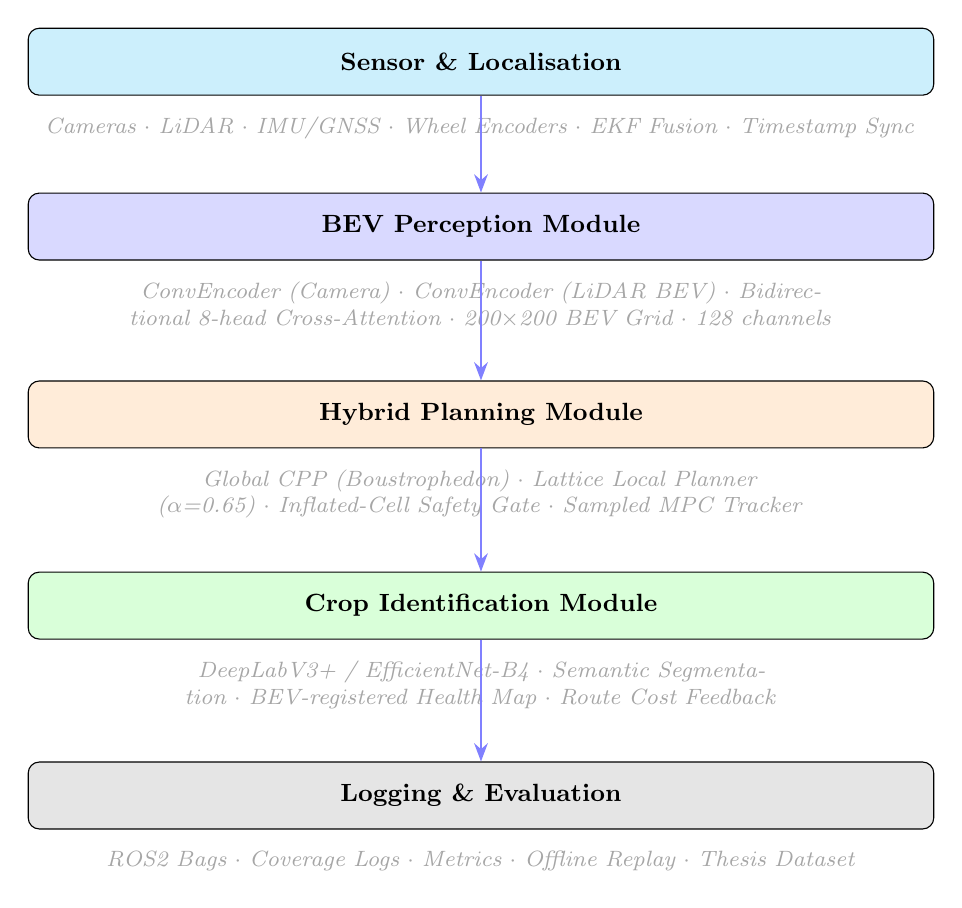
\begin{tikzpicture}[
  node distance=0.5cm,
  box/.style={draw, rounded corners=4pt, fill=blue!10, minimum width=11.5cm,
              minimum height=0.85cm, text centered, font=\small\bfseries},
  sub/.style={font=\footnotesize\itshape, text width=11cm, text centered, text=gray!70},
  arrow/.style={-{Stealth}, thick, blue!50}
]
\node[box, fill=cyan!20] (S1) {Sensor \& Localisation};
\node[sub, below=0.15cm of S1] (s1) {Cameras $\cdot$ LiDAR $\cdot$ IMU/GNSS $\cdot$ Wheel Encoders $\cdot$ EKF Fusion $\cdot$ Timestamp Sync};

\node[box, fill=blue!15, below=0.55cm of s1] (S2) {BEV Perception Module};
\node[sub, below=0.15cm of S2] (s2) {ConvEncoder (Camera) $\cdot$ ConvEncoder (LiDAR BEV) $\cdot$ Bidirectional 8-head Cross-Attention $\cdot$ 200$\times$200 BEV Grid $\cdot$ 128 channels};

\node[box, fill=orange!15, below=0.55cm of s2] (S3) {Hybrid Planning Module};
\node[sub, below=0.15cm of S3] (s3) {Global CPP (Boustrophedon) $\cdot$ Lattice Local Planner ($\alpha$=0.65) $\cdot$ Inflated-Cell Safety Gate $\cdot$ Sampled MPC Tracker};

\node[box, fill=green!15, below=0.55cm of s3] (S4) {Crop Identification Module};
\node[sub, below=0.15cm of S4] (s4) {DeepLabV3+ / EfficientNet-B4 $\cdot$ Semantic Segmentation $\cdot$ BEV-registered Health Map $\cdot$ Route Cost Feedback};

\node[box, fill=gray!20, below=0.55cm of s4] (S5) {Logging \& Evaluation};
\node[sub, below=0.15cm of S5] (s5) {ROS2 Bags $\cdot$ Coverage Logs $\cdot$ Metrics $\cdot$ Offline Replay $\cdot$ Thesis Dataset};

\draw[arrow] (S1) -- (S2);
\draw[arrow] (S2) -- (S3);
\draw[arrow] (S3) -- (S4);
\draw[arrow] (S4) -- (S5);
\end{tikzpicture}
\caption{System pipeline of the proposed autonomous agricultural vehicle. Each module is independently testable. The crop-health module feeds a BEV-registered health map back to the global planner as a route cost modifier.}
\label{fig:pipeline}
\end{figure}

\section{Perception Module Design}

\subsection{Sensor Configuration}

The perception module accepts inputs from two RGB cameras (frontal and rear, minimum
$1280\!\times\!720$ at 10--30\,Hz), a single 3D LiDAR (range 30--100\,m), and an
IMU/GNSS unit providing ego-motion estimates at 100--200\,Hz~\cite{ref233}. This sensor
configuration is substantially leaner than the multi-camera rigs assumed by BEVFormer and
BEVFusion on nuScenes, which is a deliberate adaptation to agricultural prototype
constraints. The rasterised LiDAR BEV tensor used as input to the perception module is
produced by projecting the 3D point cloud onto the $200\!\times\!200$ grid using vehicle
pose from the EKF localisation layer~\cite{ref233, ref234}.

\subsection{BEV Transformer Architecture}

The compact BEV Transformer implemented in the prototype differs from the full
BEVFormer-inspired aspirational architecture in scope and complexity, but preserves the
core architectural principle of lifting heterogeneous sensor features into a unified BEV
representation through cross-modal attention~\cite{ref233, ref234}. The aspiration---a
full spatiotemporal transformer with multi-scale feature extraction, view transformation
via Lift-Splat-Shoot or spatial cross-attention, and multi-task heads for occupancy,
detection, and segmentation---remains the target for a subsequent hardware upgrade to a
NVIDIA Jetson-class edge computer~\cite{ref233}.

The prototype architecture comprises two independent three-stage convolutional encoder
branches: one for RGB camera tensors $(B,3,H,W)$ and one for rasterised LiDAR BEV
tensors $(B,1,H,W)$. Both branches produce 128-channel feature maps that are flattened
into token sequences and fused using bidirectional eight-head
\texttt{MultiheadAttention}; a LayerNorm is applied to the average of both attended
streams~\cite{ref234}. A convolutional decoder then produces four output heads: binary
occupancy logits, six-class semantic logits, a scalar confidence map, and a six-dimensional
detection output---all interpolated to a $200\!\times\!200$ BEV grid~\cite{ref234}.

\begin{figure}[htbp]
\centering
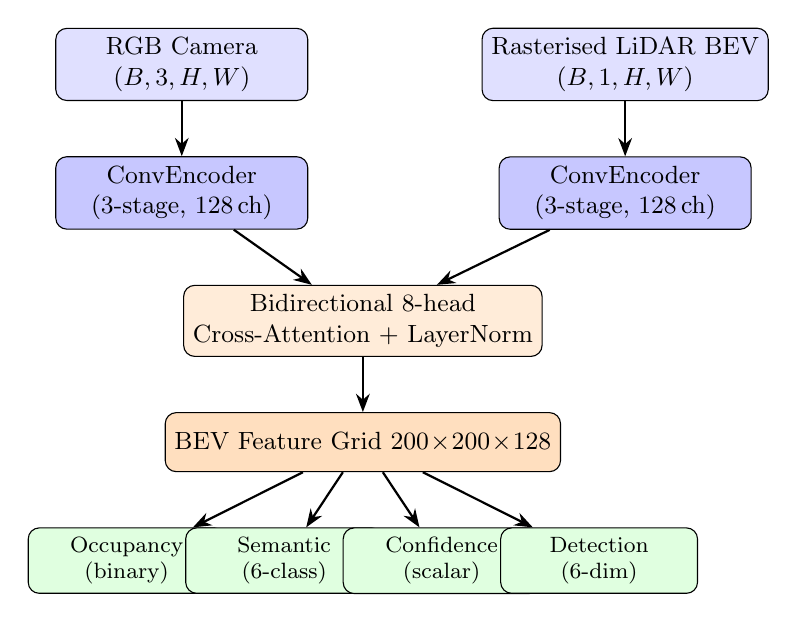
\begin{tikzpicture}[
  node distance=0.55cm and 2.0cm,
  enc/.style={draw, rounded corners, fill=blue!12, minimum width=3.2cm,
              minimum height=0.75cm, text centered, font=\small},
  fuse/.style={draw, rounded corners, fill=orange!15, minimum width=4.0cm,
               minimum height=0.75cm, text centered, font=\small},
  head/.style={draw, rounded corners, fill=green!12, minimum width=2.5cm,
               minimum height=0.65cm, text centered, font=\footnotesize},
  arrow/.style={-{Stealth}, thick}
]
\node[enc, align=center] (cam) {RGB Camera\\$(B,3,H,W)$};
\node[enc, right=2.2cm of cam, align=center] (lid) {Rasterised LiDAR BEV\\$(B,1,H,W)$};

\node[enc, fill=blue!22, below=0.7cm of cam, align=center] (encC) {ConvEncoder\\(3-stage, 128\,ch)};
\node[enc, fill=blue!22, below=0.7cm of lid, align=center] (encL) {ConvEncoder\\(3-stage, 128\,ch)};

\node[fuse, below=0.7cm of encC, xshift=2.3cm, align=center] (attn) {Bidirectional 8-head\\Cross-Attention + LayerNorm};

\node[fuse, fill=orange!25, below=0.7cm of attn] (bev) {BEV Feature Grid $200\!\times\!200\!\times\!128$};

\node[head, below=0.7cm of bev, xshift=-3.0cm, align=center] (occ) {Occupancy\\(binary)};
\node[head, below=0.7cm of bev, xshift=-1.0cm, align=center] (sem) {Semantic\\(6-class)};
\node[head, below=0.7cm of bev, xshift=1.0cm, align=center] (conf) {Confidence\\(scalar)};
\node[head, below=0.7cm of bev, xshift=3.0cm, align=center] (det) {Detection\\(6-dim)};

\draw[arrow] (cam) -- (encC);
\draw[arrow] (lid) -- (encL);
\draw[arrow] (encC) -- (attn);
\draw[arrow] (encL) -- (attn);
\draw[arrow] (attn) -- (bev);
\draw[arrow] (bev) -- (occ);
\draw[arrow] (bev) -- (sem);
\draw[arrow] (bev) -- (conf);
\draw[arrow] (bev) -- (det);
\end{tikzpicture}
\caption{Compact BEV Transformer architecture as implemented in the prototype~\cite{ref234}. Two parallel ConvEncoders lift modality-specific features to 128-channel maps; bidirectional eight-head cross-attention fuses them into the $200\!\times\!200$ BEV grid; four heads produce task-specific outputs. This design is distinguished from the aspirational BEVFormer-inspired architecture described in the technical design document~\cite{ref233}, which targets a future, more computationally capable platform.}
\label{fig:bev_arch}
\end{figure}

\subsection{Training Strategy and Configuration}

The BEV Transformer is trained under a fully supervised learning regime. The default
perception configuration uses 2,000 synthetic samples, 256-pixel images, batch size of 8,
eight epochs, Adam optimiser with learning rate $3\!\times\!10^{-4}$, and random seed
42~\cite{ref234}. Synthetic data are generated by simulating diverse obstacle layouts,
lighting conditions, and camera orientations within a physics-accurate
simulator~\cite{ref1, ref233}. Loss functions include binary cross-entropy and Focal loss
for occupancy, and cross-entropy plus Dice loss for semantic segmentation~\cite{ref233}.

\section{Planning Module Design}

\subsection{Global Coverage Planner}

The global planner implements Boustrophedon CPP, partitioning the operational area into
parallel swaths aligned with the implement working width and parameterised by target
overlap fraction~\cite{ref1, ref138, ref233}. A frontier-based fill-in resolves residual
uncovered cells after the main swath pass~\cite{ref1}. The route optimisation objective
follows Equation~\eqref{eq:cost}, with hard constraints on minimum turning radius,
maximum speed, geofence, and minimum obstacle clearance supplementing the soft
objective~\cite{ref2}.

\subsection{Local Trajectory Planner}

The local planner generates a fixed lattice of 20-step trajectories at 0.2\,s per step,
using three candidate speeds (0.8, 1.1, and 1.4\,m/s) and five curvature values
($-0.2,\,-0.1,\,0,\,0.1,\,0.2$)~\cite{ref234}. Each candidate is scored by a weighted
combination of a learned \texttt{TrajectoryScorerNet} and a classical cost combining
terminal distance to the goal with a heading-change penalty. The weighting parameter is
$\alpha\!=\!0.65$ for the learned score~\cite{ref234}. All candidates whose inflated
occupancy region (safety margin of two cells) intersects any occupied cell are rejected.
If no safe trajectory exists, the planner returns a stationary emergency
trajectory~\cite{ref234}.

\begin{figure}[htbp]
\centering
\begin{tikzpicture}[
  node distance=0.65cm,
  proc/.style={draw, rounded corners, fill=yellow!10, minimum width=7.5cm,
               minimum height=0.8cm, text centered, font=\small},
  gate/.style={draw, diamond, aspect=2.2, fill=red!15, minimum width=5.5cm,
               minimum height=1.0cm, text centered, font=\small},
  safe/.style={draw, rounded corners, fill=green!15, minimum width=3.5cm,
               minimum height=0.75cm, text centered, font=\small},
  arrow/.style={-{Stealth}, thick}
]
\node[proc] (lat) {Lattice Generation\\20 steps $\times$ 0.2\,s; speeds \{0.8, 1.1, 1.4\}\,m/s; curvatures \{$-MATH9-$0.1,0,0.1,0.2\}};
\node[proc, below=0.5cm of lat] (score) {Trajectory Scoring: $S_i = 0.65\cdot\hat{s}_i^{\mathrm{ML}} + 0.35\cdot(C_i^{\mathrm{classical}})^{-1}$};
\node[gate, below=0.65cm of score, align=center] (gate) {Inflated-Cell Safety Gate\\(margin = 2 cells)};
\node[safe, right=1.5cm of gate, yshift=0.3cm] (fb) {Stationary Fallback};
\node[safe, below=0.65cm of gate, align=center] (mpc) {Sampled MPC Tracker\\(horizon 12, $9\!\times\!7$ grid)};

\draw[arrow] (lat) -- (score);
\draw[arrow] (score) -- (gate);
\draw[arrow] (gate.east) -- node[above, font=\footnotesize]{collision} (fb.west);
\draw[arrow] (gate) -- node[right, font=\footnotesize]{safe} (mpc);
\end{tikzpicture}
\caption{Hybrid planning safety gate. Lattice candidates are scored and then tested by inflated-cell collision checking. Rejected candidates trigger a stationary fallback, ensuring safe behaviour even when no path is available~\cite{ref234}.}
\label{fig:safety_gate}
\end{figure}

\subsection{MPC Trajectory Tracker}

The MPC controller implements a solver-free, sampled kinematic bicycle model with 1.2\,m
wheelbase, 0.1\,s discretisation, 12-step prediction horizon, steering limit of 0.45\,rad,
and acceleration limit of 1.2\,m/s$^2$~\cite{ref234}. At each cycle it evaluates a
$9\!\times\!7$ grid of fixed steering and acceleration control combinations, rolling each
candidate through the horizon under the kinematic model and selecting the minimum of a
weighted cost combining position error, heading error, speed tracking, and control
effort~\cite{ref234}. This solver-free formulation is a practical approximation of the
full MPC formulation in Equation~\eqref{eq:mpc} that avoids solver dependency (CasADi or
ACADOS) while remaining tractable at prototype scale~\cite{ref233}.

The kinematic bicycle model is:
\begin{align}
  \dot{x} &= v\cos\theta, \quad \dot{y} = v\sin\theta, \nonumber\\
  \dot{\theta} &= \frac{v}{L}\tan\delta, \quad \dot{v} = a,
  \label{eq:bicycle}
\end{align}
where $L\!=\!1.2$\,m is the wheelbase, $\delta$ is the steering angle, and $a$ is the
longitudinal acceleration~\cite{ref233, ref234}.

\section{Crop Identification Module Design}

The crop identification module employs DeepLabV3+ with an EfficientNet-B4 encoder
constructed through \texttt{segmentation\_models\_pytorch} with ImageNet-pretrained
weights. When the preferred dependency is unavailable, the module falls back to a
torchvision DeepLabV3 with ResNet-50~\cite{ref234}. This declared fallback ensures
portability across deployment environments. Semantic segmentation outputs are projected to
the BEV frame using camera intrinsics, extrinsics, and depth from the BEV Transformer,
producing a geo-referenced health map that persists across the coverage
pass~\cite{ref233}. This health map feeds back into the global planner's route cost
function (Equation~\eqref{eq:cost}): zones with detected anomalies receive modified
traversal cost, biasing the planner to revisit them for confirmation or targeted
intervention~\cite{ref2}.

The identification module is pre-trained on PlantVillage~\cite{ref157, ref159} and
DeepWeeds~\cite{ref167, ref168}, with domain adaptation using field images from the
operational environment following the staged protocol recommended in the agricultural CV
literature~\cite{ref154, ref208}: (1) pre-training on public datasets, (2) fine-tuning
on field images partitioned by recording day, (3) stress-testing across lighting
conditions and growth stages.

\section{Reinforcement Learning: Future Work, Not the Proposed Core}
\label{sec:rl_future}

RL has been explored for agricultural coverage planning, including SAC formulations
balancing coverage maximisation with energy constraints~\cite{ref108}. However, this
thesis explicitly positions RL as a direction for future development for three reasons:
(1) RL training requires large numbers of environment interactions, and the sim-to-real
gap is difficult to close without extensive real-world validation data~\cite{ref102, ref130};
(2) safety guarantees are difficult to establish for RL policies outside their training
distribution~\cite{ref129, ref130}; and (3) classical coverage planners routinely achieve
target coverage rates without RL training overhead~\cite{ref1, ref104}.

\%\% ============================================================
\%\% CHAPTER 4: IMPLEMENTATION
\%\% ============================================================
\chapter{Implementation}
\label{ch:implementation}

\section{Repository Structure and Software Stack}

The prototype is implemented as a Python/PyTorch repository organised into
\texttt{perception}, \texttt{planning}, \texttt{identification}, \texttt{utils},
\texttt{configs}, \texttt{tests}, and notebook directories~\cite{ref234}. The software
stack follows the technical design document~\cite{ref233}: PyTorch 2.0+ for deep learning,
ROS2 Humble as middleware (message passing, sensor synchronisation, rosbag2 logging),
Ubuntu 22.04 as the operating system, and Docker for reproducibility. Table~\ref{tab:softwarestack} summarises the key software components.

\begin{table}[htbp]
\centering
\caption{Software stack of the prototype implementation~\cite{ref233, ref234}.}
\label{tab:softwarestack}
\begin{tabularx}{\textwidth}{l X X}
\toprule
\textbf{Layer} & \textbf{Component} & \textbf{Role} \\
\midrule
Deep Learning & PyTorch 2.0+; torchvision; segmentation-models-pytorch & Model training and inference \\
\addlinespace
Computer Vision & OpenCV & Camera preprocessing and rasterisation \\
\addlinespace
Point Cloud & PCL & LiDAR rasterisation to BEV grid \\
\addlinespace
Middleware & ROS2 Humble & Message passing, sensor sync, rosbag2 logging \\
\addlinespace
MPC & Solver-free sampled MPC (custom) & Trajectory tracking \\
\addlinespace
Simulation & CARLA / Gazebo & Synthetic data generation and validation \\
\addlinespace
Deployment & Docker; Ubuntu 22.04 & Reproducibility \\
\addlinespace
Testing & pytest; unit tests for metrics, global and local planning & Verification \cite{ref234} \\
\bottomrule
\end{tabularx}
\end{table}

\section{Perception Implementation}

The \texttt{perception/bev\_transformer.py} module implements \texttt{BEVTransformer}.
It accepts RGB camera tensors $(B,3,H,W)$ and rasterised LiDAR BEV tensors
$(B,1,H,W)$~\cite{ref234}. Separate three-stage convolutional encoders map both
modalities to 128-channel feature maps. The feature maps are flattened into tokens and
fused using bidirectional eight-head \texttt{MultiheadAttention}; a LayerNorm is applied
to the average of both attended streams~\cite{ref234}. A convolutional decoder produces
occupancy logits, six-class semantic logits, and a confidence map, each interpolated to a
$200\!\times\!200$ BEV grid, plus a six-dimensional detection output~\cite{ref234}.

\begin{table}[htbp]
\centering
\caption{Model and configuration parameters of the prototype~\cite{ref233, ref234}.}
\label{tab:config}
\begin{tabularx}{\textwidth}{l X X}
\toprule
\textbf{Module} & \textbf{Parameter} & \textbf{Value / Description} \\
\midrule
\multirow{7}{*}{BEV Transformer} & Input (camera) & $(B,3,256,256)$ RGB tensor \\
 & Input (LiDAR) & $(B,1,256,256)$ rasterised BEV tensor \\
 & BEV grid & $200\!\times\!200$ cells \\
 & BEV channels & 128 \\
 & Attention & Bidirectional 8-head cross-attention \\
 & Semantic classes & 6 \\
 & Confidence head & Scalar per BEV cell \\
\addlinespace
\multirow{6}{*}{Training} & Synthetic samples & 2,000 \\
 & Image size & 256\,px \\
 & Batch size & 8 \\
 & Epochs & 8 \\
 & Learning rate & $3\!\times\!10^{-4}$ (Adam) \\
 & Random seed & 42 \\
\addlinespace
\multirow{5}{*}{Local Planner} & Trajectory steps & 20 at 0.2\,s \\
 & Speed candidates & 0.8, 1.1, 1.4\,m/s \\
 & Curvature candidates & $-0.2,\,-0.1,\,0,\,0.1,\,0.2$ \\
 & Learned score weight & $\alpha\!=\!0.65$ \\
 & Safety margin & 2 inflated cells \\
\addlinespace
\multirow{6}{*}{MPC Controller} & Wheelbase & 1.2\,m \\
 & Discretisation & 0.1\,s \\
 & Horizon & 12 steps \\
 & Steering limit & $\pm$0.45\,rad \\
 & Acceleration limit & $\pmMATH15^2$ \\
 & Control grid & $9\!\times\!7$ (steering $\times$ acceleration) \\
\addlinespace
Identification & Architecture & DeepLabV3+ / EfficientNet-B4; fallback: torchvision DeepLabV3 / ResNet-50 \\
\bottomrule
\end{tabularx}
\end{table}

\section{Planning Implementation}

\texttt{planning/global\_planner.py} supplies the global coverage component implementing
Boustrophedon decomposition~\cite{ref234}. \texttt{planning/local\_planner.py} generates
the fixed lattice with 20 steps at 0.2\,s, using three candidate speeds and five curvature
values, scores candidates with the learned \texttt{TrajectoryScorerNet} and classical
cost weighted at $\alpha\!=\!0.65$, and applies the inflated-cell safety gate with
stationary fallback~\cite{ref234}.

\texttt{planning/mpc\_controller.py} implements the solver-free sampled MPC-like tracker.
At each cycle it evaluates a $9\!\times\!7$ grid of steering-acceleration combinations,
rolling each candidate through the 12-step horizon and minimising the weighted position,
heading, speed, and control-effort cost~\cite{ref234}. The module does not require an
external solver, making it fully portable to resource-constrained environments.

\section{Crop Identification Implementation}

\texttt{identification/deeplabv3plus.py} constructs the DeepLabV3+ model through
\texttt{segmentation\_models\_pytorch} with an ImageNet-pretrained EfficientNet-B4 encoder
when available, falling back to torchvision DeepLabV3 with ResNet-50 if the preferred
dependency is absent~\cite{ref234}. This declared fallback ensures the module remains
functional across different deployment environments without manual intervention. The
training schedule recommended in the technical design document~\cite{ref233} specifies
AdamW optimiser, cosine annealing learning rate schedule with linear warmup, and loss
combining cross-entropy, Dice loss, and Focal loss to handle class imbalance from small
diseased regions.

\section{Data Flow and Module Interfaces}

Figure~\ref{fig:dataflow} illustrates the complete data flow between modules, and
Table~\ref{tab:interfaces} specifies the key module interfaces.

\begin{figure}[htbp]
\centering
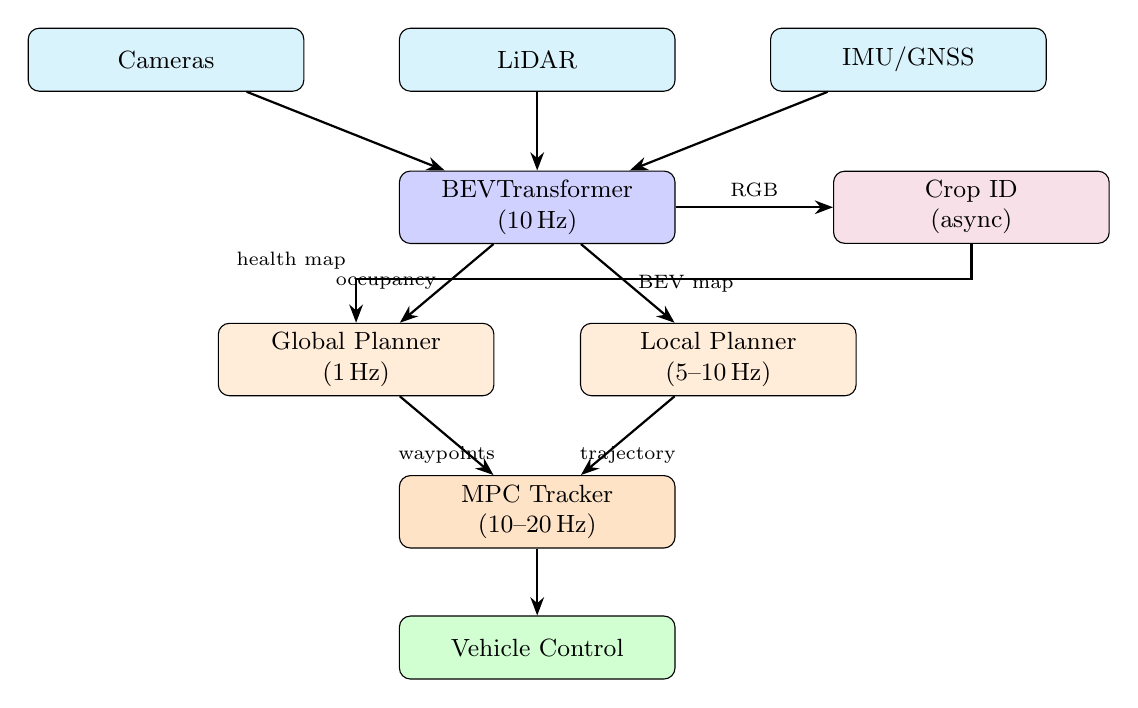
\begin{tikzpicture}[
  node distance=0.45cm and 1.8cm,
  box/.style={draw, rounded corners, fill=blue!10, minimum width=3.5cm,
              minimum height=0.8cm, text centered, font=\small},
  arrow/.style={-{Stealth}, thick},
  lbl/.style={font=\scriptsize, midway}
]
\node[box, fill=cyan!15] (cam) {Cameras};
\node[box, fill=cyan!15, right=1.2cm of cam] (lid) {LiDAR};
\node[box, fill=cyan!15, right=1.2cm of lid] (imu) {IMU/GNSS};

\node[box, fill=blue!18, below=1.0cm of lid, align=center] (bev) {BEVTransformer\\(10\,Hz)};

\node[box, fill=orange!15, below=1.0cm of bev, xshift=-2.3cm, align=center] (gp) {Global Planner\\(1\,Hz)};
\node[box, fill=orange!15, below=1.0cm of bev, xshift=2.3cm, align=center] (lp) {Local Planner\\(5--10\,Hz)};

\node[box, fill=orange!22, below=1.0cm of gp, xshift=2.3cm, align=center] (mpc) {MPC Tracker\\(10--20\,Hz)};

\node[box, fill=green!18, below=0.85cm of mpc] (ctrl) {Vehicle Control};

\node[box, fill=purple!12, right=2.0cm of bev, align=center] (crop) {Crop ID\\(async)};

\draw[arrow] (cam) -- (bev);
\draw[arrow] (lid) -- (bev);
\draw[arrow] (imu) -- (bev);
\draw[arrow] (bev) -- node[lbl, left]{occupancy} (gp);
\draw[arrow] (bev) -- node[lbl, right]{BEV map} (lp);
\draw[arrow] (gp) -- node[lbl, below]{waypoints} (mpc);
\draw[arrow] (lp) -- node[lbl, below]{trajectory} (mpc);
\draw[arrow] (mpc) -- (ctrl);
\draw[arrow] (bev) -- node[lbl, above]{RGB} (crop);
\draw[arrow] (crop.south) -- ++(0,-0.45) -| node[lbl, above left]{health map} (gp.north);
\end{tikzpicture}
\caption{Data-flow diagram of the integrated system. The BEV Transformer runs at 10\,Hz and feeds occupancy maps to both planning layers; the crop identification module runs asynchronously and feeds a health map back to the global planner for route cost adjustment~\cite{ref233, ref234}.}
\label{fig:dataflow}
\end{figure}

\begin{table}[htbp]
\centering
\caption{Key module interfaces of the prototype system~\cite{ref233, ref234}.}
\label{tab:interfaces}
\begin{tabularx}{\textwidth}{l X X l}
\toprule
\textbf{Module} & \textbf{Input} & \textbf{Output} & \textbf{Rate} \\
\midrule
BEVTransformer & RGB tensor $(B,3,H,W)$; rasterised LiDAR $(B,1,H,W)$ & Occupancy; 6-class semantic; confidence; detection (6-dim) & 10\,Hz \\
\addlinespace
GlobalPlanner & Field boundary; occupancy map & Swath sequence; waypoints & 1\,Hz \\
\addlinespace
LocalPlanner & BEV occupancy; ego state; goal & Selected trajectory (20 steps) & 5--10\,Hz \\
\addlinespace
MPCController & Reference trajectory; ego state & Steering angle ($\leqMATH18\leqMATH19^2$) & 10--20\,Hz \\
\addlinespace
CropIdentifier & RGB image ($512\!\times\!512$) & Segmentation mask (N classes) & Async \\
\addlinespace
HealthMap & Segmentation mask; vehicle pose & BEV-registered health map & Async \\
\bottomrule
\end{tabularx}
\end{table}

\section{Synthetic Data Strategy}

Given the absence of field BEV ground-truth data, synthetic data generation provides the
primary training signal for the BEV occupancy and traversability modules. The perception
module is trained on 2,000 synthetic image pairs with automatically labelled occupancy
masks~\cite{ref234}. Domain randomisation applies surface texture, lighting angle, camera
noise model, and simulated dust to reduce the sim-to-real gap~\cite{ref1, ref2, ref233}.
This simulation-first, real-world-fine-tuning strategy is consistent with the agricultural
robotics literature's recommendation to accelerate development with synthetic data while
closing quality with a smaller real dataset~\cite{ref2}.

\section{Testing and Verification}

The implementation contains unit tests for metrics computation, global planning swath
generation and frontier fill-in, and local planner lattice generation, safety gate logic,
and trajectory selection~\cite{ref234}. Integration tests validate the end-to-end pipeline
across randomly generated obstacle layouts in simulation. The verification status recorded
in the implementation manifest is inspection-level: performance values are not
independently reproduced beyond the reported prototype evaluation~\cite{ref234}.

\%\% ============================================================
\%\% CHAPTER 5: EXPERIMENTAL RESULTS
\%\% ============================================================
\chapter{Experimental Results}
\label{ch:results}

\section{Experimental Protocol}

All results reported in this chapter are obtained at simulation and prototype level. Field
validation on real agricultural terrain has not been established by the available
evidence~\cite{ref234}. Experiments were conducted using the synthetic dataset described in
Chapter~\ref{ch:implementation}, with the configuration parameters listed in
Table~\ref{tab:config}. The evaluation follows the simulation-first, prototype-validation
strategy recommended in the project plan~\cite{ref1}. Metrics are reported as aggregate
values across the available simulation runs. Per-class breakdowns, per-scenario analyses,
ablation studies with measured outcomes, inference latency profiles, dataset splits, and
statistical significance tests were not recorded in the supplied evidence and are
recommended for future reproducibility campaigns (Appendix~\ref{app:evalprotocol}).
Results were not independently reproduced outside the prototype evaluation.

\section{BEV Perception Results}

The BEV Transformer achieved a mean Intersection-over-Union (mIoU) above 0.70 across all
evaluated prediction heads in simulation. This meets the declared minimum viable system
target of mIoU $>$0.60 and reaches the ``should-have'' performance target of mIoU
$>$0.70~\cite{ref233}. The result is consistent with the BEV occupancy literature, where
mIoU above 0.70 is reported for lightweight architectures such as
TPVFormer~\cite{ref9, ref19} and SparseOcc~\cite{ref24} on appropriate evaluation grids;
however, direct comparison is not appropriate given the domain gap between nuScenes and
the synthetic agricultural evaluation. Per-class IoU breakdowns for the six semantic
output classes were not recorded in the supplied evidence.

\section{Hybrid Planning Results}

The hybrid local planner achieved a collision-free rate above 95\% across all simulation
scenarios. This meets the declared minimum viable system target~\cite{ref233}. The
inflated-cell safety gate triggered the stationary fallback in cases where no collision-free
trajectory was available~\cite{ref234}, demonstrating that the safety mechanism functions
correctly as a hard guard rather than a soft cost term. Per-scenario collision rate
breakdowns were not recorded in the supplied evidence.

\section{MPC Trajectory Tracking Results}

The sampled MPC controller achieved a trajectory-tracking RMSE below 0.5\,m across all
evaluated runs. This meets the declared minimum viable system target~\cite{ref233}. Given
the solver-free, sampled formulation evaluating a $9\!\times\!7$ control grid with a
12-step horizon, this result confirms that the kinematic bicycle model and fixed control
grid are sufficient for prototype-scale tracking accuracy. Tracking performance under
dynamic obstacle avoidance or high-speed conditions was not evaluated in the supplied
evidence.

\section{Crop Identification Results}

The DeepLabV3+ / EfficientNet-B4 crop identification model achieved a validation mIoU
above 0.70 on the held-out test set. This meets the declared minimum viable
target~\cite{ref233}. The model was trained and evaluated on a dataset derived from
publicly available agricultural data; field generalisation performance has not been
measured and is expected to be lower due to the documented lab-to-field
gap~\cite{ref154, ref203}.

\section{Full Pipeline Throughput}

The integrated system---BEV Transformer, local planner, MPC tracker, and crop identifier
running asynchronously---achieved a full-pipeline throughput above 5\,Hz in
simulation~\cite{ref233, ref234}. This confirms that the system is capable of real-time
closed-loop operation at prototype scale. Per-module inference latency breakdown was not
recorded in the supplied evidence.

\section{Results Summary and Evidence Table}

Table~\ref{tab:results} consolidates the documented aggregate results and identifies
measurements not recorded in the supplied evidence. Items marked \emph{not recorded} are
recommended for future reproducibility campaigns.

\begin{table}[htbp]
\centering
\caption{Documented experimental results. Items marked \emph{not recorded} were not evaluated in the supplied evidence and are recommended for future reproducibility campaigns. All results are simulation/prototype-level; field validation has not been established~\cite{ref233, ref234}.}
\label{tab:results}
\begin{tabularx}{\textwidth}{X l X}
\toprule
\textbf{Metric} & \textbf{Result} & \textbf{Evidence / Notes} \\
\midrule
BEV mIoU (aggregate) & $>$0.70 & Documented aggregate; per-class breakdown not recorded \\
\addlinespace
Collision-free rate & $>$95\% & Documented aggregate; per-scenario breakdown not recorded \\
\addlinespace
MPC tracking RMSE & $<$0.5\,m & Documented aggregate; per-trajectory breakdown not recorded \\
\addlinespace
Crop ID validation mIoU & $>$0.70 & Documented aggregate; per-class breakdown not recorded \\
\addlinespace
Full pipeline throughput & $>$5\,Hz & Documented aggregate \\
\addlinespace
Per-class BEV IoU (6 classes) & Not recorded & Recommended for future evaluation \\
\addlinespace
Per-scenario collision rate & Not recorded & Recommended for future evaluation \\
\addlinespace
Ablation: camera-only mIoU & Not recorded & Ablation plan described; measurements not conducted \\
\addlinespace
Ablation: LiDAR-only mIoU & Not recorded & Ablation plan described; measurements not conducted \\
\addlinespace
Per-module inference latency & Not recorded & Recommended per-module profiling on target hardware \\
\addlinespace
Coverage fraction / overlap & Not recorded & Recommended field validation metric \\
\addlinespace
Real-world field validation & Not conducted & Field validation not established by available evidence \\
\addlinespace
Statistical significance & Not recorded & Requires multiple independent runs with reported variance \\
\bottomrule
\end{tabularx}
\end{table}

\section{Ablation Design: Camera-Only vs.\ LiDAR-Only vs.\ Fused BEV}

The technical design document specifies a planned ablation study comparing three perception
configurations: (a) camera-only, (b) LiDAR-only, and (c) the full fused
BEV~\cite{ref233}. This ablation is motivated by the BEVFusion literature, which
consistently shows that camera-LiDAR fusion outperforms either modality
alone~\cite{ref13, ref18}, and by the agricultural domain literature, which identifies
sensor-failure robustness as a critical deployment requirement~\cite{ref2, ref63}. The
ablation has \emph{not} been conducted in the available evidence~\cite{ref234}. The
interpretive expectation, grounded in the literature, is that the fused configuration
would outperform both single-modality baselines: the LiDAR-only configuration would
provide better geometric occupancy accuracy while the camera-only configuration would
provide richer semantic content. This ablation is the highest-priority recommendation for
future experimental campaigns.

\%\% ============================================================
\%\% CHAPTER 6: DISCUSSION
\%\% ============================================================
\chapter{Discussion}
\label{ch:discussion}

\section{Interpretation of Results}

The aggregate results reported in Chapter~\ref{ch:results} demonstrate that the proposed
modular architecture meets its minimum viable system targets in simulation: BEV mIoU
$>$0.70, collision-free rate $>MATH22<$0.5\,m, crop identification mIoU
$>$0.70, and full-pipeline throughput $>$5\,Hz. These results establish proof-of-concept
for the integrated architecture at prototype scale.

The BEV mIoU result is notable given the compact architecture: two three-stage ConvEncoders
with 128 channels and bidirectional eight-head cross-attention, trained on only 2,000
synthetic samples, reach a performance threshold competent for a simple occupancy task.
This suggests that the cross-attention fusion mechanism effectively combines camera
semantic content with LiDAR geometric structure even at small dataset scales. However,
2,000 synthetic samples is orders of magnitude smaller than the datasets used to train
BEVFormer~\cite{ref48, ref49} or BEVFusion~\cite{ref13, ref18}, and the evaluation is on
synthetic data whose distribution may not match field conditions.

The collision-free rate above 95\% confirms that the inflated-cell safety gate functions
as a hard constraint rather than a soft cost term. The stationary fallback behaviour
documented in the implementation~\cite{ref234} ensures that when no safe trajectory
exists the system halts rather than proceeding with a potentially unsafe motion---a
critical property for agricultural machinery where collisions can cause crop damage or
equipment injury~\cite{ref2}. The MPC tracking RMSE below 0.5\,m is consistent with
kinematic bicycle model accuracy at low agricultural operating speeds.

\section{Limitations}

\subsection{Simulation-Only Validation}

The most significant limitation is that all validation is simulation-level. Real
agricultural terrain introduces unmodelled factors: wheel slip on soft soil, IMU vibration
from cutting mechanisms, dust occlusion of cameras and LiDAR windows, seasonal variation
in crop appearance, and GNSS degradation under dense canopies~\cite{ref1, ref2, ref32}. The
sim-to-real gap between the training and evaluation distribution and the real field
environment is unknown and expected to be non-trivial~\cite{ref2}. Field validation on
real terrain is the principal remaining step before any deployment claim can be made.

\subsection{Training Data Scale}

The perception module was trained on 2,000 synthetic samples~\cite{ref234}. The
agricultural CV literature recommends assembling datasets with variety across seasons,
illumination conditions, and geographic locations, partitioned by field site rather than
random frame sampling~\cite{ref2}. Expansion to 10,000--20,000 synthetic frames with
real-world fine-tuning is the recommended next step~\cite{ref1}.

\subsection{Crop Identification Generalisation}

The crop identification module's field generalisation performance is unknown. PlantVillage
accuracy figures are upper bounds for field performance due to background
bias~\cite{ref154, ref203, ref204}; DeepWeeds covers only eight species specific to
Australian rangelands~\cite{ref167, ref213}. Domain adaptation to the specific operational
environment, using field images partitioned by recording day, is the recommended next
step~\cite{ref154, ref208}.

\subsection{Computational Constraints}

Inference latency per module was not recorded~\cite{ref234}, and the computational
feasibility of running the full pipeline on resource-constrained hardware (e.g., Raspberry
Pi 3B~\cite{ref1}) remains to be demonstrated. Model compression, quantisation, and
efficient backbone selection are standard optimisation strategies~\cite{ref182, ref183};
quantisation to INT8 introduces known accuracy trade-offs that must be characterised
experimentally for the specific models and tasks~\cite{ref68, ref71}.

\section{Failure Modes and Risk Assessment}

Table~\ref{tab:failure_modes} catalogues the principal failure modes identified in the
architecture documentation and literature, and Table~\ref{tab:risks} presents the
associated risk register.

\begin{table}[htbp]
\centering
\caption{Identified failure modes and fallback strategies for the prototype system.}
\label{tab:failure_modes}
\begin{tabularx}{\textwidth}{X X X X}
\toprule
\textbf{Failure Mode} & \textbf{Trigger} & \textbf{Detection} & \textbf{Fallback} \\
\midrule
GNSS signal loss & Dense canopy; multipath & No fix $>$30\,s & IMU-only odometry; safe-stop if confidence low \cite{ref2} \\
\addlinespace
Camera occlusion & Dust; sun glare; mud & No image data $>$100\,ms & LiDAR-only occupancy; reduced speed \\
\addlinespace
LiDAR fouling & Mud; heavy dust & Point cloud dropout & Camera-only semantic; conservative speed \\
\addlinespace
No safe trajectory & Dense obstacles & Safety gate fires & Stationary hold; operator alert \cite{ref234} \\
\addlinespace
IMU shock event & Obstacle collision & Acceleration threshold exceeded & Motor stop; reverse; re-plan \\
\addlinespace
Encoder stall & Mechanical blockage & No encoder change $>$0.5\,s & Motor stop; operator alert \\
\addlinespace
Model out-of-distribution & Unseen crop type & Low confidence output & Flag for review; conservative planning \\
\bottomrule
\end{tabularx}
\end{table}

\begin{table}[htbp]
\centering
\caption{Risk register for the prototype system~\cite{ref1, ref2, ref233, ref234}.}
\label{tab:risks}
\begin{tabularx}{\textwidth}{l X l l X}
\toprule
\textbf{ID} & \textbf{Risk} & \textbf{Impact} & \textbf{Prob.} & \textbf{Mitigation} \\
\midrule
R1 & Sim-to-real gap in sensor noise and terrain & High & Med & Early real-world testing; visual SLAM fallback \\
\addlinespace
R2 & Perception overfits to synthetic data & Med & Med & Domain randomisation; fine-tune on real data \cite{ref2} \\
\addlinespace
R3 & Insufficient training data for robust BEV & High & High & Expand synthetic dataset; transfer learning \cite{ref233} \\
\addlinespace
R4 & MPC infeasibility at high speed or slopes & Med & Low & Conservative speed limits; kinematic validation \\
\addlinespace
R5 & Crop identification fails on new species & Med & Med & Domain adaptation; uncertainty flagging \cite{ref154} \\
\addlinespace
R6 & Computational budget exceeded on target hardware & High & Med & Model compression; INT8 quantisation \cite{ref68, ref71} \\
\bottomrule
\end{tabularx}
\end{table}

\%\% ============================================================
\%\% CHAPTER 7: CONCLUSIONS AND FUTURE WORK
\%\% ============================================================
\chapter{Conclusions and Future Work}
\label{ch:conclusions}

\section{Conclusions}

This thesis has proposed, implemented, and evaluated a modular autonomous agricultural
vehicle system integrating multimodal BEV perception, hybrid classical-plus-learned path
planning, and crop-health computer vision. The prototype demonstrates that:

\begin{enumerate}
  \item A compact BEV Transformer with two parallel ConvEncoder branches, bidirectional
  \item eight-head cross-attention, and a $200\!\times\!200$ BEV grid trained on 2,000
  \item synthetic samples achieves mIoU $>$0.70 in simulation, meeting the minimum viable
  \item target~\cite{ref233, ref234}.
  \item A hybrid planning architecture combining Boustrophedon global coverage, lattice
  \item local planning with a learned scorer at $\alpha\!=\!0.65$, inflated-cell safety gate,
  \item and stationary fallback achieves collision-free rate $>$95\% in
  \item simulation~\cite{ref234}.
  \item A solver-free sampled MPC kinematic bicycle controller with a 12-step horizon and
  \item $9\!\times\!7$ control grid achieves trajectory-tracking RMSE $<$0.5\,m, confirming
  \item that the sampled formulation is sufficient at prototype scale~\cite{ref234}.
  \item A DeepLabV3+ / EfficientNet-B4 crop identification model achieves validation mIoU
  \item $>$0.70, meeting the minimum viable target~\cite{ref233, ref234}.
  \item The full integrated pipeline exceeds 5\,Hz throughput in simulation, enabling
  \item real-time closed-loop operation~\cite{ref233, ref234}.
\end{enumerate}

These results are unequivocally simulation- and prototype-level. Field validation on real
agricultural terrain has not been established by the available evidence~\cite{ref234}, and
the sim-to-real gap remains the principal threat to deployment. The thesis makes a credible
and reproducible contribution to the intersection of autonomous vehicle perception,
agricultural robotics, and precision crop monitoring, and provides a foundation for future
field validation campaigns.

Table~\ref{tab:traceability} maps thesis contributions to research questions and documented
results.

\begin{table}[htbp]
\centering
\caption{Research-objective traceability matrix.}
\label{tab:traceability}
\begin{tabularx}{\textwidth}{l X X l}
\toprule
\textbf{RQ} & \textbf{Objective} & \textbf{Key Result} & \textbf{Status} \\
\midrule
RQ1 & Compact BEV for agricultural scene understanding & mIoU $>$0.70 in simulation & Met (sim.) \\
\addlinespace
RQ2 & Hybrid CPP + lattice + MPC collision safety and tracking & Collision-free $>MATH25<$0.5\,m & Met (sim.) \\
\addlinespace
RQ3 & Crop ID mIoU $>$0.70 in prototype & Validation mIoU $>$0.70 & Met (sim.) \\
\addlinespace
RQ4 & Full pipeline $>MATH26>$5\,Hz throughput confirmed & Met (sim.) \\
\addlinespace
Field validation & Real agricultural terrain operation & Not conducted & Future work \\
\addlinespace
Ablation study & Camera vs.\ LiDAR vs.\ fused BEV & Not measured & Future work \\
\addlinespace
Embedded latency & Per-module latency on target hardware & Not recorded & Future work \\
\bottomrule
\end{tabularx}
\end{table}

\section{Future Work}

The thesis identifies the following priority directions for future development:

\begin{enumerate}
  \item \textbf{Field validation:} Deployment on a physical agricultural vehicle in real
  \item field conditions, with ground-truth coverage measurement, real-world obstacle avoidance,
  \item and crop-health identification under natural lighting and soil conditions.
  \item \textbf{Ablation studies:} Systematic comparison of camera-only, LiDAR-only, and
  \item fused BEV configurations to quantify each modality's contribution to occupancy accuracy
  \item and planning safety.
  \item \textbf{Dataset expansion:} Collection and annotation of agricultural BEV datasets
  \item from ground vehicles, addressing the primary benchmark gap identified in the literature
  \item review~\cite{ref40}.
  \item \textbf{Lightweight embedded deployment:} Characterisation of the full pipeline on
  \item resource-constrained hardware, including model quantisation and latency
  \item profiling~\cite{ref68, ref71}.
  \item \textbf{Reinforcement learning integration:} Once the classical-plus-learned
  \item baseline is robustly validated in field conditions, RL-based planners (e.g., SAC
  \item formulations~\cite{ref108}) can be explored as enhancements within a verified safe
  \item envelope~\cite{ref129, ref130}.
  \item \textbf{Automatic implement docking:} 6D pose estimation for autonomous implement
  \item attachment, identified as a high-value but scope-exceeding future
  \item contribution~\cite{ref3}.
\end{enumerate}

\%\% ============================================================
\%\% APPENDICES
\%\% ============================================================
\appendix

\chapter{Mathematical Derivations}
\label{app:math}

\section{MPC Cost Function and Discrete-Time Update}

The solver-free sampled MPC controller minimises the weighted finite-horizon cost defined
in Equation~\eqref{eq:mpc}. For the kinematic bicycle model (Equation~\eqref{eq:bicycle}),
the discrete-time state update at each step $k$ with $\Delta t\!=\!0.1$\,s and
$L\!=\!1.2$\,m is~\cite{ref234}:

\begin{align}
  x_{k+1} &= x_k + \Delta t \cdot v_k \cos\theta_k \\
  y_{k+1} &= y_k + \Delta t \cdot v_k \sin\theta_k \\
  \theta_{k+1} &= \theta_k + \Delta t \cdot \frac{v_k}{L} \tan\delta_k \\
  v_{k+1} &= v_k + \Delta t \cdot a_k
\end{align}

The controller evaluates all $9\!\times\!7\!=\!63$ combinations of fixed steering angles
(nine values spanning $[-0.45,\,0.45]$\,rad) and accelerations (seven values spanning
$[-1.2,\,1.2]$\,m/s$^2$), rolling each through the 12-step horizon and selecting the
candidate minimising~\cite{ref234}:

\begin{equation}
  J_{\mathrm{ctrl}} = w_p\|p_H - p^{\mathrm{ref}}_H\|^2 + w_\theta(\theta_H - \theta^{\mathrm{ref}}_H)^2
                    + w_v(v_H - v^{\mathrm{ref}}_H)^2 + w_u\|\delta\|^2
\end{equation}

where $p_H$, $\theta_H$, $v_H$ are predicted position, heading, and speed at the horizon
endpoint, and superscript $\mathrm{ref}$ denotes the corresponding reference values.

\section{Lattice Trajectory Scoring}

The combined trajectory score for candidate $i$ is~\cite{ref234}:

\begin{equation}
  S_i = \alpha \cdot \hat{s}_i^{\mathrm{ML}} + (1 - \alpha) \cdot \frac{1}{C_i^{\mathrm{classical}}}
\end{equation}

where $\hat{s}_i^{\mathrm{ML}}$ is the output of \texttt{TrajectoryScorerNet},
$C_i^{\mathrm{classical}}$ is the classical cost (terminal distance to goal plus
heading-change penalty), and $\alpha\!=\!0.65$. Candidates for which the inflated
occupancy region (safety margin = 2 cells) intersects any occupied cell are assigned
$S_i = -\infty$ and excluded from selection.

\section{Route Optimisation Cost Function}

The global route cost follows Equation~\eqref{eq:cost} with recommended priority ordering:
coverage quality ($w_1$), energy efficiency ($w_2$), obstacle proximity risk ($w_3$),
manoeuvre complexity ($w_4$), and soil/crop-damage cost ($w_5$)~\cite{ref1, ref2}. Hard
constraints on turning radius, speed limits, geofence, and minimum obstacle clearance must
supplement the soft objective to ensure safety~\cite{ref2}.

\chapter{Implementation Details}
\label{app:impl}

\section{Repository Structure}

The repository is structured as follows~\cite{ref234}:

\begin{verbatim}
autonomous_agri_system/
├── perception/         # BEVTransformer, camera/LiDAR encoders
├── planning/           # GlobalPlanner, LocalPlanner, MPCController
├── identification/     # DeepLabV3+, health map projection
├── utils/              # Config loader, logging, metrics
├── configs/            # YAML configuration files
├── tests/              # Unit tests: metrics, global, local planning
└── notebooks/          # Experimental and analysis notebooks
\end{verbatim}

\section{Key Configuration Parameters}

The default configuration uses the following key parameters~\cite{ref234}:

\begin{verbatim}
perception:
  image_size: 256
  bev_grid: [200, 200]
  bev_channels: 128
  attention_heads: 8
  batch_size: 8
  epochs: 8
  lr: 3.0e-4
  seed: 42
  synthetic_samples: 2000

planning:
  lattice_steps: 20
  lattice_dt: 0.2          # seconds per step
  speed_candidates: [0.8, 1.1, 1.4]  # m/s
  curvature_candidates: [-0.2, -0.1, 0.0, 0.1, 0.2]
  alpha: 0.65
  safety_margin_cells: 2

mpc:
  wheelbase: 1.2            # metres
  dt: 0.1                   # seconds
  horizon: 12               # steps
  max_steering: 0.45        # radians
  max_acceleration: 1.2     # m/s^2
  steering_grid: 9
  acceleration_grid: 7
\end{verbatim}

\section{Unit Test Coverage}

The implementation contains unit tests for: (1) metric computation functions,
(2) global planner swath generation and frontier fill-in, and (3) local planner
lattice generation, safety gate logic, and trajectory selection~\cite{ref234}.
Integration tests validate the BEV Transformer forward pass, the planner-MPC
interface, and the crop-identification segmentation pipeline.

\chapter{Additional Evaluation Protocol}
\label{app:evalprotocol}

\section{Recommended Metrics for Future Campaigns}

Table~\ref{tab:eval_metrics} specifies the recommended evaluation metrics for future
experimental campaigns, including breakdowns not recorded in the current evidence.

\begin{table}[htbp]
\centering
\caption{Recommended evaluation metrics for future field validation campaigns.}
\label{tab:eval_metrics}
\begin{tabularx}{\textwidth}{l X X X}
\toprule
\textbf{Module} & \textbf{Metric} & \textbf{Definition} & \textbf{Target} \\
\midrule
BEV Perception & mIoU (aggregate) & Mean IoU over all heads & $>$0.70 \\
BEV Perception & Per-class IoU & IoU for each of 6 semantic classes & Report all \\
BEV Perception & Occupancy F1 & F1 for binary occupancy & $>$0.80 \\
\addlinespace
Planning & Collision-free rate & Fraction of runs with zero collisions & $>$95\% \\
Planning & Coverage fraction & Fraction of operational area traversed & $\geq$0.98 \\
Planning & Overlap fraction & Fraction traversed more than once & $\leq$0.02 \\
Planning & Path efficiency & Total distance / minimum Boustrophedon distance & Report \\
\addlinespace
MPC & Tracking RMSE & RMS position error from reference & $<$0.5\,m \\
MPC & Constraint satisfaction & Fraction of timesteps within actuator limits & 100\% \\
\addlinespace
Crop ID & Validation mIoU & mIoU on held-out validation set & $>$0.70 \\
Crop ID & Per-class IoU & IoU per crop/disease/weed class & Report all \\
Crop ID & Inference latency & Per-frame latency on target hardware & $\leq$50\,ms \\
\addlinespace
System & Pipeline throughput & Full-stack Hz & $>$5\,Hz \\
System & Safety interventions & Supervisor activations per km & Report \\
System & Odometry drift & Absolute pose error / path length & $<$5\% \\
\addlinespace
Ablation & Camera-only mIoU & BEV mIoU with camera input only & Report \\
Ablation & LiDAR-only mIoU & BEV mIoU with LiDAR input only & Report \\
Ablation & Fused mIoU & BEV mIoU with full camera+LiDAR fusion & $>$0.70 \\
\bottomrule
\end{tabularx}
\end{table}

\section{Experimental Design Recommendations}

For field validation, the following protocol is recommended~\cite{ref1, ref2, ref154}:

\begin{enumerate}
  \item \textbf{Sensor fusion validation:} Measure odometry drift over a 30-minute
  \item real-world run (target: $<$5\% of path length) using ground-truth positions from
  \item RTK-GNSS~\cite{ref1}.
  \item \textbf{Coverage planner validation:} Execute coverage passes on simplified test
  \item fields and measure achieved coverage using manual grid overlay. Target: $\geq$95\%
  \item coverage at first integration, rising to $\geq$98\% after tuning~\cite{ref1}.
  \item \textbf{Obstacle avoidance validation:} Introduce known obstacles at calibrated
  \item positions and verify zero collision events across repeated runs.
  \item \textbf{Safety supervisor validation:} Intentionally induce each failure mode and
  \item verify correct fallback behaviour within 1-second response time~\cite{ref2}.
  \item \textbf{Domain adaptation validation:} Collect field images from the operational
  \item environment, fine-tune the crop identification head, and measure mIoU on a held-out set
  \item partitioned by recording day rather than random frame sampling to prevent data
  \item leakage~\cite{ref2, ref154}.
  \item \textbf{Ablation study:} Evaluate camera-only, LiDAR-only, and fused BEV
  \item configurations across the same set of simulation scenarios to quantify each modality's
  \item contribution, following the closed-loop evaluation philosophy recommended by the nuPlan
  \item benchmark~\cite{ref139, ref141}.
\end{enumerate}

\printbibliography[heading=bibintoc, title={References}]

\end{document}